\chapter{Ensemble Methods and the Naive Bayes Classifier}\label{ch:ensembleMethods}

This chapter begins with formulations and introductory discussions of the most common tree-based classifiers, and finishes with the formulation of the Naive Bayes learner.
For all of these models, we will present their advantages and disadvantages as predictors, along with a comparison of the model's performance.
This assessment will compare models' benefits and drawbacks in a specific long-term migration experiment using processed CDR data.

\section{Classifier: Decision Trees}\label{section:decision_trees}


% The models builds a
Decision trees are models that can be understood as a tree-like graph structures in which each node of the tree contains a conditional statement. 
These conditional statemnts act as a rules which split input samples in a binary relationshipo of two disjoint sets.
In this way, we have that at each node samples split in two possible branches which recursively continue to further nodes which again split the samples.
 % any input data sample can comply or not.
The rules are propositions or statements that are eigher true or false and they are built as a linear (or similar) binary partition over feature space. 
In the algorithmic implementation each rule will be defined by assigning a threshold for a given feature which splits samples over those above and below this threshold.
In this way, at each node the model evaluates each input sample $x$ with the proposition by checking if $x^j \in U$, where $x^j$ is the feature used for that node's rule and $U$ is a subset of the feature's domain.
After the split, the algorithm recursively partitions each of the resulting splits with another rule. 
 % decision forwards it to one of the possible remaining partitions 
 % to create a binary partition of the data.
% over a single feature threshold for every sample.
%properties of the values for each feature.


For numerical features, the input space $X$ will be partitioned into $L$ and $R$, namely left and right, where $L$ takes the form $(-\infty,d]$. The value $d \in \mathbb{R}$ is a number predefined by the rule itself and is actually computed by the algorithm during the optimization procedure.
In the same way, for categorical features $L$ will be a subset of the possible category values for that feature.

By iterating this process over more nodes, a tree defines a partition of feature space in multiple regions $A_1,\ldots,A_K$.
Here the number of iterations $K \in \mathbb{N}$ is a hyperparameter which is dependent on the algorithm's convergence criterion.
Each region will have an associated value $c_k$ in such a way that the tree's predicted output $\hat{y}$, for a sample $x$, is $c_k$, when the sample belongs to $A_k$.
Here $c_k$ will be one of the possible values taken by the target variable $y$ in the training set.
If we take into consideration the way trees are built, we will have that each $A_k$ is a hyper-rectangle in feature space.

\subsection{Decision Trees Formulation}\label{subsection:decision_trees_formulation}
In short, the learner can be characterized by the following formula:
\begin{equation}
\label{eq:decisionTreeModel}
h(X) = \sum_{k=1}^K c_k I(X \in A_k)
\end{equation}

where $c_k$ is the output value that our model estimates for samples in the $A_k$ region.
Both of these will have to be learned by the model during optimization. %by minimizing its loss function

By the principles given above, the algorithm will need to determine an ``optimal'' way to split a set of samples, that flow through a decision node.
In this learner, the \textit{goodness of splits} are measured by specific functions called \textit{node impurity measures}.
Later in \cref{subsection:decision_trees_impurity_measures} we give specific examples of node impurity measures.
%them according, in order to optimize a loss metric.

%at each node
Most variations for this Machine Learning model build rules (tree nodes) in a sequential, greedy, fashion, where node impurity measures are locally optimized at each node to decide on which is the best splitting value.
The reason for doing this is because the construction of optimal binary decision trees is NP-Complete~\citep{decisionTreesNP}.
Doing otherwise would result in an algorithm whose computational complexity is infeasible.

At any splitting node we have to find the \textit{best} feature $X^j \ / j \in \ [1, \ldots, p] $ and value split $d$ for which to partition the data in
$$A_L(d,j) = \{x \in \mathcal{T} \ / \ x^j \leq d \} $$
and
$$A_R(d,j) = \{x \in \mathcal{T}\ / \ x^j> d \} $$

Let $N_l$ and $N_r$ be $|A_L|$ and $|A_R|$ respectively and note that we have taken $(p,j)$ as given. 
However, the Decision Tree algorithm will find both in an optimization routine.
To quantify the \textit{best} feature $j \in \ [1, \ldots, p]$ for this split, the algorithm will minimize:

%\frac{1}{N_{left}}
%\frac{1}{N_{right}}

\begin{equation}
\label{eq:decisionTreeGreedyOptimization}
%\begin{split}
\min_{j,d} \big[ \min_{c_L }  \frac{1}{N_l}\sum_{x \in A_L(d,j) } L(y,c_L)    \ +  \min_{c_R}  \frac{1}{N_r}\sum_{x \in A_R(d,j) } L(y,c_R) \big]
%\end{split}
\end{equation}

where $y$ is the target associated to the samples $x$ that are part of that node's split. 
Also, $L(\cdot)$ is the loss function used by the algorithm to measure the quality of the split in this optimization.
Note that this can be done efficiently for a wide range of loss functions since the minimization can be done for each feature independently.

A tree is then grown in an iterative way from the top down\footnote{In this context the \textit{top} of a tree refers to the root of the tree.}, estimating the appropriate parameters at each rule split.
All of the training set's samples would start at the top (the root node) and then travel down through the tree's branches, where at each step the node's rul will decide to what branch below does the sample move to.
A branch of the tree would stop growing once the samples at a node have reached a certain \textit{purity} i.e. when samples belong to the same class.
Other stopping criteria include halting when a minimum number of samples has been reached.

We would finally have that the tree's leafs are the partition subsets over the input data and, once a tree is built, predicting targets for new samples is straightforward: the prediction of their target class will be the value given after traveling the sample down to its corresponding leaf node.

To illustrate a constructed tree using this method, an instance of a grown tree is shown in \cref{fg:rf-treeFigure}.
This classification tree example is built from a dummy gender prediction problem, using CDRs as input data. 
We must note here that there is not much interpretability in this toy example:
%[.{\textit{Woman}}]
\smallskip
\begin{figure}[h]
\Tree[.{ $Calling\_Volume \leq 23$ } [.{$Province \in \{ San Luis, Chubut \} $} [.{$Time\_Weekend \geq 16$} [.{\textit{M}} ] [.{\textit{F}} ] ]
[.{$Calls\_Weekdays \leq 48$}
[.{ $Time\_Weekday \geq 17$} [.{\textit{M}} ] [.{\textit{F}} ]] [.{\textit{F}} ] ] ]
[.{$Calls\_Mondays \geq 2$} [.{$Province \in \{ Chubut, Cordoba \} $} [.{\textit{M}} ] [.{\textit{F}} ] ]
[.{\textit{M}} ]]]
\caption{Classification tree example built for a toy gender prediction problem, using CDR available data.}
\label{fg:rf-treeFigure}
\end{figure}

\smallskip


%[.{\textit{M}} ] [.{\textit{F}} ]

\subsection{Impurity Measures}\label{subsection:decision_trees_impurity_measures}


The most used metrics to build each rule are the \textit{Gini impurity measure} and the \textit{entropy} or \textit{information gain} criterion.
The former minimizes the misclassification error in the output sets that result from the partition.
It optimizes the model's accuracy as the resulting score of tagging all the leaf's samples with the majority label in that partition.

The latter measure optimizes for information entropy, which is analogous to minimizing \textit{Kullback-Leibler divergence} of the resulting sets with respect to the original set prior to the split.

In addition, we have the misclassification measure.
Following is listed formulation of the these three impurity measures for classification trees:

\begin{itemize}
    \item Gini index: $ \displaystyle \sum_{k\neq k'} \hat{p}_{jk} \hat{p}_{jk'}  = \sum_{k=1}^{K} \hat{p}_{jk} (1 - \hat{p}_{jk}) $
    \item Cross-entropy: $ \displaystyle \sum_{k=1}^{K} -\log(\hat{p}_{jk})\hat{p}_{jk} $
    \item Misclassification error: $ \displaystyle \frac{1}{N_j} \sum_{x \in R_j} I(y\neq c_j) = 1 - c_j $
\end{itemize}

% In some cases, a reweighted Gini index can be efficient where in this version a loss matrix is used to multiply each summand of the measure.
% By this, the matrix reassigns weights to different cases of misclassification.
% This practice become specifically relevant when we have that a sample from class $k$ incorrectly assigned to class $k'$ is more valuable than other misclassifications.
% Let $L \in \mathbb R_{\ge 0}^{K \times K}$ where $L_{(k,k')}$ is the cost of misclassifying a class $k$ sample into $k'$.
% Naturally we will have $L$ as a null diagonal matrix.
% As such, the Gini index's summands will take the reweighed form $L_{kk'} \hat{p}_{jk} \hat{p}_{jk'}$.

For the case of binary (two class) classification, these measures can be expressed in simpler terms.
If we consider $p$ to be the probability of success, then we have

\begin{itemize}
\item Misclassification binary error: $1 - max(p, 1-p)$ \label{it:decisionTreeCostFunctions}
\item Gini binary index: $ 2p(1-p) $
\item Binary cross-entropy: $ -\log(p)p - \log(1- p)(1-p) $
\end{itemize}


\subsection{Hyperparameters}\label{subsection:decision_trees_hyperparameters}

For the decision tree model, the process of iteratively partitioning the samples in splits continues until a predefined tuning parameter stops the optimization or when the node is pure i.e.\ there is only a single target class for all samples at the node.

The hyper-parameters for this model includes the length of the tree, the splitting rule threshold and the node impurity measures.
From the descriptions previously given, we can list these directly:

\begin{itemize}
\item Max depth of the tree, or the allowed levels of splits.
\item The criteria or measure used to select the best split feature at each node.
\item The leaf size or the total number of minimum samples allowed per leaf.
Note that this is a related to limit on branch depth.
\item Number of features selected to decide on the best split feature at each node.
\end{itemize}


Intuitively, it is natural to find that trees of longer depth will overfit the data since more complex interactions among variables will be captured by refining the input space partition.
A trivial example is to allow a tree to grow fully in depth to later assign all training set's samples to their own self-contained regions.
This will yield a model with virtually zero bias yet with a very high prediction error.

In \cref{figure:dtree_overfit_problem_2} we give an overfit decision tree example, using the  \cref{target2} problem of tagging outward migrants of the endemic region.
It is clear that the overly-complex model produces poor generalization error.
%Recall that this was described in \cref{figure:dtree_overfit_problem_2}.
Here the training and CV scores were both compared on models with increasing tree depth.
We see how at some point, the learner started to overfit the training set where this is reflected in the gap between the CV and training errors.

At the same time, having a tree which is too shallow in depth will result in a biased algorithm  for most cases.
This is because it results in an overly simple model incapable of correctly assigning labels.
We must then consider that the depth of a tree is a measure of the model's complexity and as such, one of the most important hyperparameters of our model.

Another drawback of the decision tree model is the high variance instability.
Authors point out that two very similar datasets can grow two very different resulting trees.
This is due to the hierarchical nature of the splits, where errors randomly made in the first splits will be carried later on.
Once a sample has been directed through a lower branch, it will continue down through this one without reconsideration of the past errors.

For the reasons described, in this model it is important to control the depth of the trees built.
To do this, the most common method for doing this grows a very large tree $T_0$ that will continue until it reaches a depth limit threshold that is very nonrestrictive.
Then the tree will be pruned by removing branches and nodes to lower the model's complexity whilst at the same time trying not to compromise much of its accuracy.
More details on this can be seen in \cref{appx:sec:tree_pruning}.
For a broad characterization of decision trees and their construction in classification or regression problems, please refer to~\citep{breiman-cart84}.

\subsection{Experiment}\label{subsection:decision_trees_experiment}

We present here a run of a decision tree over $\mathcal{T}$.
Again, the case the \cref{target2} was used as an example, where we intend to correctly tag those TelCo users which were living in the endemic region in $T_0$ and then migrated to $T_1$.

The tree was built using a standard configuration with a low depth of 5 and a Gini splitting criteria.
At each decision node, we configured the algorithm to be able to select any feature $X^j$ to perform the split.
Also, we configured the minimum split threshold to be of $20$ samples.
This meant that no further splits were created when less than this number of samples was left at that node.
Under this setup, the algorithm ran in approximately 15 seconds.
\cref{fig:decision_tree_actual_problem} shows a partial representation of the actual decision tree grown on \cref{target2}.
This allows us to see how the algorithm selects better features at low-level nodes, versus the deeper splits.

% \bigskip

\clearpage

\begin{sidewaysfigure}[H]
    \centering
    \makebox[\textwidth]{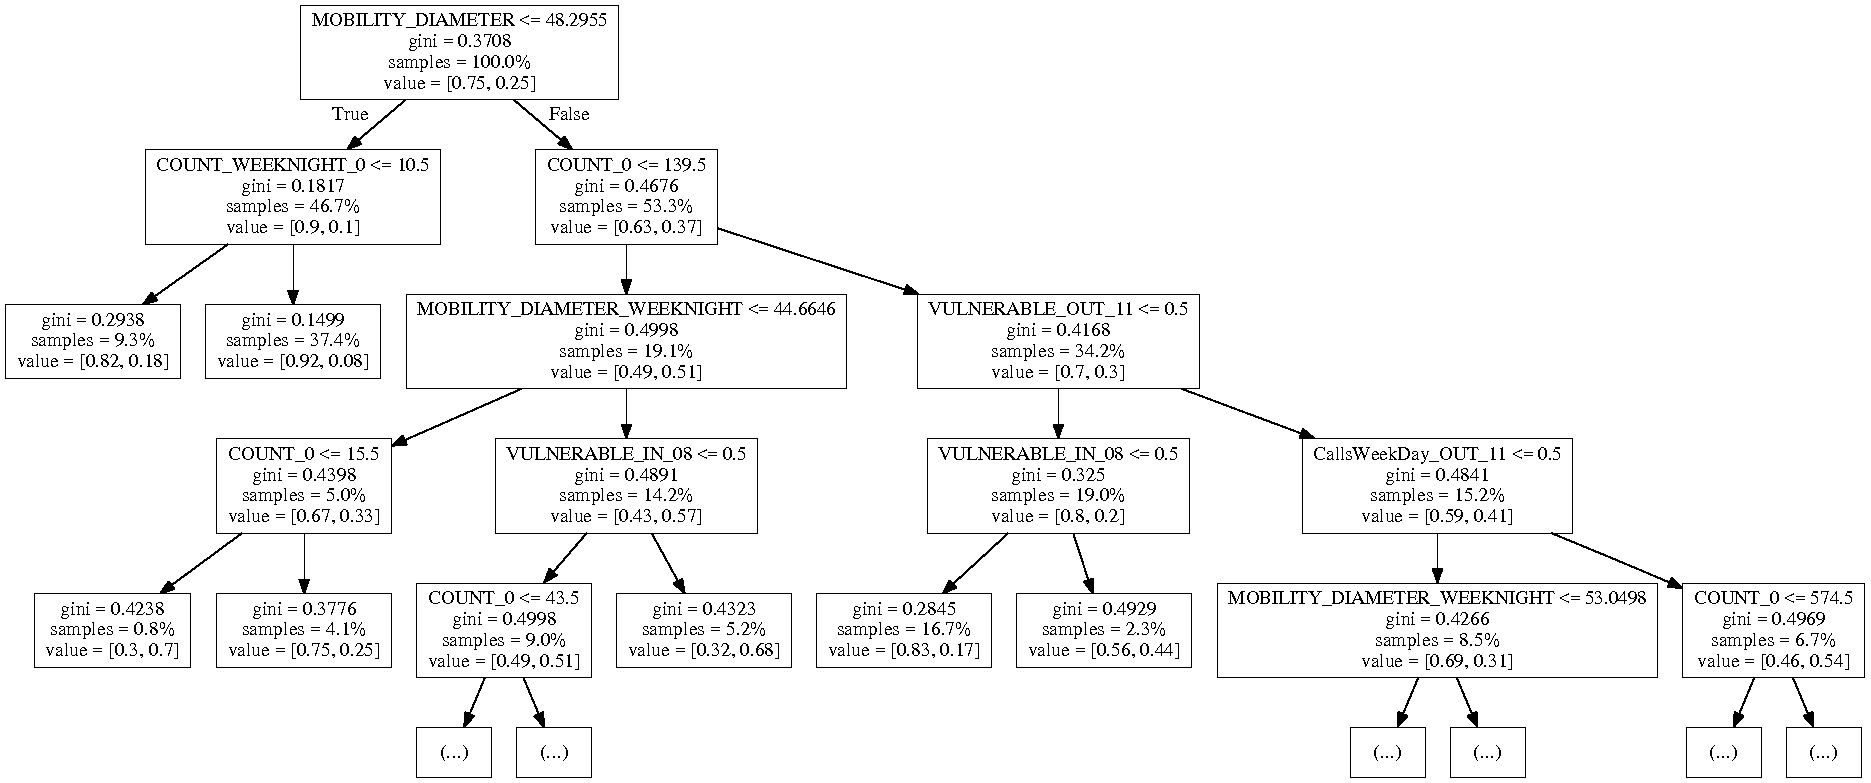
\includegraphics[width=1.2\paperwidth]{figures/decision_tree/full_tree_map.png}}
    \caption{ Example of a final decision tree.
        This model was made with a cross validated procedure on \cref{target2} and the resulting tree has been pruned to fit the image.
        For every node, the samples are split into sets given by the implicit indicator function defined in the condition.}
    \label{fig:decision_tree_actual_problem}
\end{sidewaysfigure}



%\begin{figure*}[tb]
%\centering
% \makebox[\textwidth]{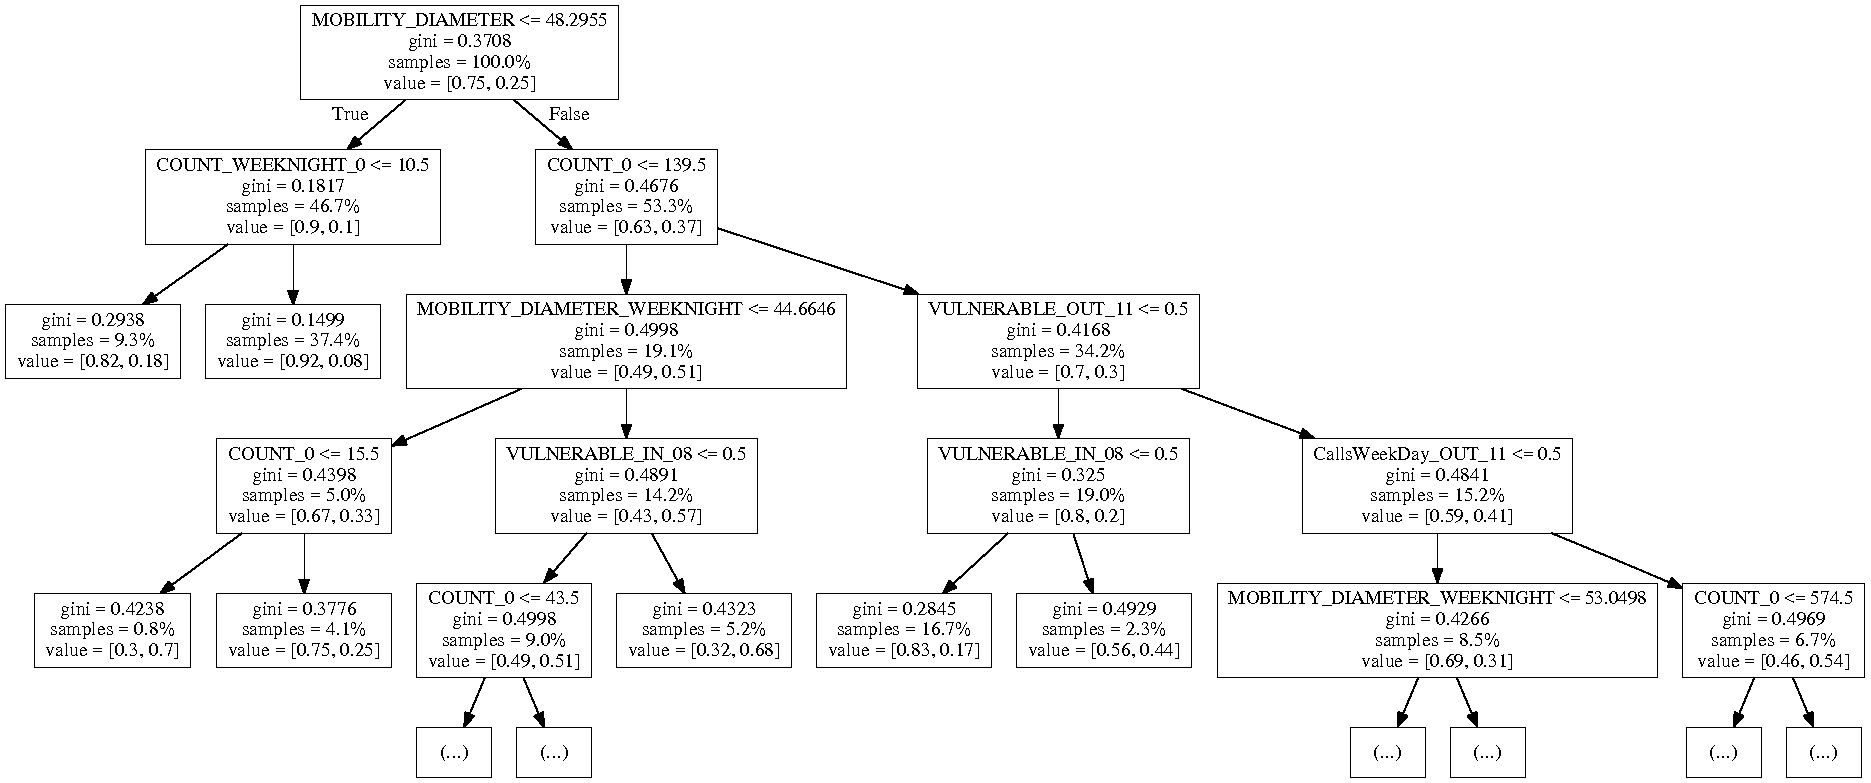
\includegraphics[width=.9\paperwidth]{figures/decision_tree/full_tree_map.png}}
%\caption{ Example of a final decision tree. This model was made with a cross validated procedure on \cref{target3} and the resulting tree has been pruned to fit the image. For every node, the samples are split into sets given by the implicit indicator function defined in the condition.}
%\label{fig:decision_tree_actual_problem}
%\end{figure*}

% \smallskip


From \cref{fig:decision_tree_actual_problem} we can approximate which features are most important to the algorithm when deciding a node split, given by the Gini splitting criteria.
Given that in \cref{target2} we are looking for people that migrated out of the endemic region, the choice of the tree's root feature seems appropriate.
The mobility diameter gives an idea of a user's influence area when using their mobile phone and as such, this attribute might indicative of past migrations.
Subsequently, the usage volume of a user's home antenna appears as the second most important features, both during weeknights and for the whole day.

The error score reached by this tree, however, yields a low performance over all of the samples because if we evaluate the learner with the $Accuracy$ metric, we see a classification score of $43.2\%$.
Under these circumstances, noting which features were selected near the root leaves of the tree can be misleading if we do not recheck these results.
In this way we decide to iterate this model one more time, but now choosing to change some hyperparameter values.
For this time, we set control the target class imbalance in the training set $\mathcal{T}$.
As we have noted beofre, the positive and negative classes have a disproportionate balance of samples and this has direct impact in the overall model's poor performance.
To help tackle this imbalance, we modify the tree's loss function's setup to assign higher weight to samples of the under-represented class and underweight the samples from the abundant group.
We will have that for each sample, its loss weight was adjusted by its class representation ratio and, with this, the new run scored a $57.9\%$ $Accuracy$  which is more than a $15\%$ increase over the previous score.
The figure for this model is shown in \cref{fig:decision_tree_actual_problem2}.
% Still, this is considered a very poor model for supervised learning.


% \bigskip
\clearpage

\begin{sidewaysfigure}[H]
    \centering
    \makebox[\textwidth]{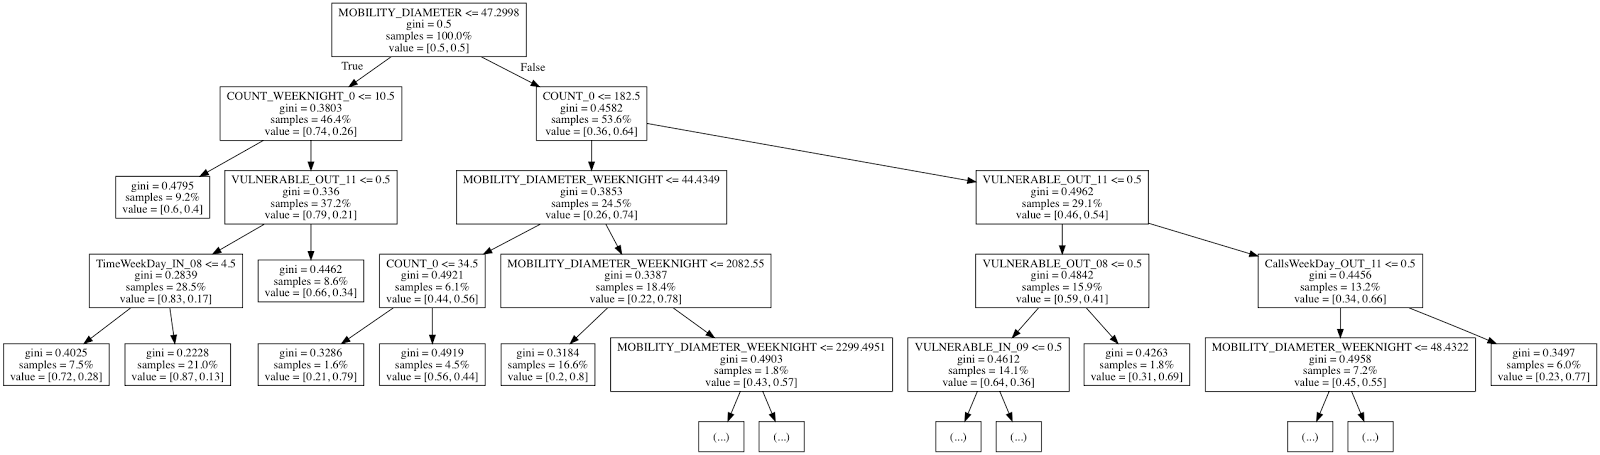
\includegraphics[width=1.2\paperwidth]{figures/decision_tree/full_tree_map2.png}}
    \caption{ Second example of a decision tree.
        This model was made with a cross validated procedure on \cref{target2} from an artificially balanced dataset.
        The resulting tree has been pruned to fit the image.}
    \label{fig:decision_tree_actual_problem2}
\end{sidewaysfigure}


% \clearpage

The importance of the mobility diameter becomes clearer in \cref{fig:decision_tree_actual_problem2}.
Once again the learner selects this attribute as the first split in the data, and this time with balanced samples.
Recall that by the stochastic nature of the algorithm constructing the tree, two runs with the same hyperparameter settings and data need not output the same trees.
In this case however, it is notable that the final tree still uses the mobility feature in the first split in the data, even with balanced samples.
And the same can be said of the feature representing the count of calls made from the home antenna.

This tree has a better performance than before yet it has an average performance in its prediction of which users have migrated in the past.
At some point, it is reasonable to assume that balancing classes leads to a better predictive outcome yet there are still various misclassifications in the predicted target classes.
If we let the tree grow deeper though, we might increase the performance of the training error as shown in \cref{figure:dtree_overfit_problem_2}.
But again, this won't help our generalization error.
So to tackle most of the disadvantages described by this technique, \textit{Random Forests} are what follow as a natural extension to this classifier.

\section{ Random Forests}\label{section:random_forests}

Random Forests are estimators that extend from constructing a group of single decision trees and then combining them to produce a single output decision.
This grouping of classifiers is known as an \textit{ensemble}.

The objective in this construction is to focus on decision tree's low bias whilst controlling their overfit as much as possible.
For this, a forest of single trees will be constructed in such a way that correlations among each of the individual models is limited.
The idea behind this is to have every individual model train on a random subset of features or samples and then, average the single outputs as the forest's target output.
With this we preserve single estimator's interdependence as much as possible.
There are other different techniques that intent to construct uncorrelated trees which are combined at the output, yet the main idea is common to all.

\subsection{ Random Forests Formulation}\label{subsection:random_forests_formulation}

Let $K$ be the number of trees in the ensemble and let $\Theta_k$ encode the parameters for the $k$-th tree.
As we have mentioned before, there are various variants to the model and these variants will define the type of encoding for the $\Theta_k, k \in {1,\ldots,K}$  parameters.
For the following part, we will not specify the specific ensembly type constructed since the formulation is common to all of them.

To begin, we define
$$h(\textbf{x},\Theta_k)$$ as the corresponding individual classifier and we let $N$ be the number of samples in the training set $\mathcal{T}$.
The creation of a random forest involves an iterative procedure where at the $k$-th step, the parameter $\Theta_k$ is fit from the same distribution as $\Theta_j, \ j<k$, yet it is built in a way that is independent of the previous parameters $\{\Theta_1, \ \ldots, \ \Theta_{k-1} \}$. %$\Theta$ will be encoded by a vector of randomly drawn integers from 1 to $M$ which is part of the model's hyperparameters.


Let $\{ h_k(\textbf{x}) \}_{i=1}^K$\footnote{There is an abuse of notation by noting trees as $h_k(\textbf{x})$ and not $h(\textbf{x}, \Theta_k)$ } be a set of classifying trees and let $I(\cdot)$ denote the indicator function.

Define the margin function as

\begin{equation}
\label{eq:rf-marginFun}
mg(\textbf{x},\textbf{y}) = \frac{1}{K}  \sum_{k=1}^K I(h_k(\textbf{x}) = \textbf{y})
- \max_{j\neq \textbf{y}}\left(\frac{1}{K} \sum_{k=1}^K I(h_k(\textbf{x}) = j) \right)
\end{equation}


This function measures, in average, how much do the trees vote for the correct class in comparison to all other classes and it is the training error of the model when using the misclassification loss.
Here the generalization error is denoted as $PE*$ and is equal to

\begin{equation}
P_{\textbf{x}, \textbf{y} }(mg(\textbf{x},\textbf{y}) <0)
\end{equation}

 It can be shown that, for $K$ sufficiently large, the generalization error under the misclassification loss converges to

\begin{equation}
 P_{\textbf{x}, \textbf{y} } ( P_{\Theta} (h(\textbf{x}, \Theta) = \textbf{y}) - \max_{j \neq \textbf{y}} P_{\Theta} (h(\textbf{x}, \Theta) = j) < 0)
 \end{equation}

almost surely for all sequences of parameters $\Theta_1,\Theta_2, \ldots, \Theta_k,\ldots$

This proof can be found in \cref{appx:sec:rforest_margin_function_convergence}.


\subsection{ Experimental comparison to Decision Trees}\label{subsection:random_forests_comparison_trees}

From what is formulated in \cref{subsection:random_forests_formulation} and in order to compare how this model improves over the Decision Tree model, we ran two experiment setups on a Random Forest learner for the difficult  \cref{target2}.
We selected the $Accuracy$ score to measure the learner's performance.
The model was trained in a cross validation procedure of 10 folds for each configuration, and in each experiment we optimized the score for a different model hyperparameter.

For the first experiment, we evaluated the forest's scores on a maximum depth variation for the trees.
And on the second one, we tried to illustrate the point of \cref{subsection:random_forests_formulation} by considering forests of increasing size.
As a default configuration, we set both the trees' max depth and the number of trees to 10.

Also, we pre-configure a balanced weighting of positive and negative samples in the loss function, where each sample is weighted by the reciprocal of the class's ratio to the whole dataset.
Finally, the impurity measure we used was the Gini index for the splitting criteria at each tree's node.

Cross validation procedures ran for 1412.8 and 2506.1 seconds respectively.
In both of them we excluded any user attributes that informed their home state and current endemic condition, in the time period $T_1$.

The experiment's scores outcomes across their hyperparameter values were graphed in \cref{fig:random_forest_validation_curves_depth_trees,fig:random_forest_validation_curves_num_trees}.
For both, the cross-validated and training set scores were compared. In this way, for each hyperparameter value, the $1-Accuracy$ score is shown.
In this way, having a lower score in the graphic means a better model was reached.

\begin{figure}[h!]
    \begin{center}
     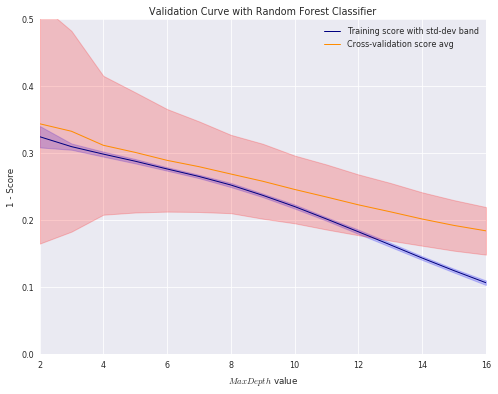
\includegraphics[width=1\linewidth]{figures/random-forest/validation_curve_forest_depth_series_f1}
        \caption{ Validation curve on the tree-depth hyperparameter values for the Random Forest  learner.
            The mean CV scores for the $1 - Accuracy$ score is shown for a CV run experiment on \cref{target2}}
        \label{fig:random_forest_validation_curves_depth_trees}

    \end{center}
\end{figure}

\begin{figure}[h!]
    \begin{center}
        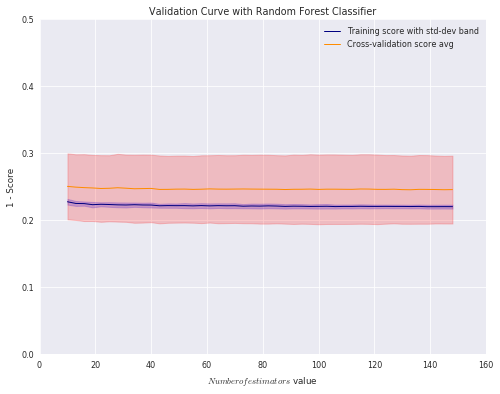
\includegraphics[width=1\linewidth]{figures/random-forest/validation_curve_forest_num_trees_series_f1}
            \caption{ Validation curve on the number of trees hyperparameter values, for the Random Forest  learner.
                The mean CV scores for the $1 - Accuracy$ score is shown for a CV run experiment on \cref{target2}}
        \label{fig:random_forest_validation_curves_num_trees}
    \end{center}
\end{figure}

Recall how this relates to \cref{figure:dtree_overfit_problem_2}, in which a tree's training error always improves as a result of an increase in the tree's depth.
Yet we saw how the tree's generalization error starts to suffer and deteriorate at one point.

From what we can see in \cref{fig:random_forest_validation_curves_depth_trees}, the cross validated error is always decreasing for increasing tree depth.
A very slight deceleration in the decrease of the cross validated error can be seen for tree depth bigger than 9.
However scores keeps improving and don't worsen.
This is different to \cref{figure:dtree_overfit_problem_2} where if we let the tree grow deeper, at one point we only worsen the performance of the test error.
Here, we are possibly improving the generalization error, as indicated by the CV estimation.

 On the other hand, it is interesting to note that there is an insignificant decrease in the training and CV scores when the number of trees is increased.
For this case, there is virtually no change in model error by improving bias or variance.

An explanation for this might that we are setting a default tree depth of 10 levels already when running this experiment.
And a tree configuration of this type might then be capturing all the possible model complexity to this dataset.
Another plausible explanation for this is that, for this task, the forest's performance rapidly converges to the generalization error with a minimum of 10 trees and that adding more trees doesn't certainly improve on the predictions.

At their optimal configuration, both setups reached CV score averages of at least $75\%$, with a maximum of $81\%$ for the forest
with trees of 16 levels.
The optimal number of estimators for the CV and the training sets were not the same though, where 139 was the best configuration for the training score whilst 133 was the best average for the CV set.
The relative difference in these best scores was of $3.3\%$.

At the same time, the relative difference of the best CV and training scores, for the maximum tree depth experiment was of $9.5\%$.
This percentage difference signals that the max depth hyper-parameter is significantly more sensible to over-fitting than the number of trees used.


\subsection{Predictive error bounds}\label{subsec:rforest_predictive_error_bounds}

Random Forests are built upon a bag of weaker classifier, of which each individual estimator has a different prediction error.
To build an estimate of the generalization error on the ensemble classifier, these individual scores and the relationship between them must be measured.
In this sense, the \textit{strength} and \textit{correlation}of a Random Forest must be analyzed to arrive on an estimate of the generalization error.

Define $$\hat{\jmath}( \textbf{x},\textbf{y}) = \argmax_{j \neq \textbf{y}} P_{\Theta}(h(\textbf{x}) = j)$$

and let the margin function for a random forest (not a group of classifiers) be defined as

\[
mr(\textbf{x},\textbf{y}) = P_{\Theta}(h(\textbf{x}) = \textbf{y}) - P_{\Theta}(h(\textbf{x}) = \hat{\jmath})
\\
= \Expect_{\Theta} \left[ I(h(\textbf{x},\Theta ) = y ) - I( h( \textbf{x},\Theta ) = \hat{\jmath} ) \right]
\]

This characterizes the expectation taken over another function which is called the \textbf{raw margin function}.
Intuitively, the raw margin function takes each sample to be $1$ or $-1$ according to whether the ensemble classifier can correctly classify or not the sample's label, given the ensemble's structure specified by $\Theta$.

With this, we can introduce the strength for this forest as

\begin{equation}
s = \Expect_{\textbf{x},\textbf{y}} \left[ mr(\textbf{x},\textbf{y} ) \right]
\end{equation}

Now define $ \rho(\Theta, \Theta')$ as the correlation between $rmg(\Theta,\textbf{x},\textbf{y})$ and $rmg(\Theta',\textbf{x},\textbf{y})$ of two learners, then we can have the mean value correlation for the ensemble as

%   where we have conveniently defined as
%Note that this is the mean value of the correlation.
\begin{equation}
\overline{\rho} = \frac{\Expect_{\Theta, \Theta'} \left[ \rho(\Theta, \Theta') \sigma(\Theta) \sigma(\Theta')\right]}
{\Expect_{\Theta, \Theta'} \left[ \sigma(\Theta) \sigma(\Theta')\right]}
\end{equation}

With the above we can then see that,

\begin{theorem}
There exists an upper bound for the generalization error of a Random Forest which is    \begin{equation}
PE^* \leq \overline{\rho}\frac{(1-s^2)}{s^2}
\end{equation}
\end{theorem}

The proof of this can be found in \cref{appx:sec:rforest_predictive_error_bounds}.\\

This bound on the generalization error shows the importance of each individual weak classifier's strength to the forest's generalization error, and the correlation interdependence among them.

This proof was first introduced in~\citep{breiman-randomforests} and there, it is said that the bound may not be tight enough for practical significance.
Special importance is also put on the ratio between base learner's correlation and strength ($\frac{\overline{\rho}}{s^2}$).
It is know that, to build a strong classifier, this should be as small as possible.
For this reason decision trees make a canonical choice for weak learners, being low biased models which are prone to overfitting.
These ensembles are a first choice when building a first, cost-effective, model to deliver a prediction task with acceptable to excellent performance.


\subsection{Other Notes on Random Forests}\label{subsection:random_forests_other_notes}

One benefit of building Random Forest classifiers is that the algorithm can easily increase a group of estimators' prediction error by randomly building every specific learner in a way that decreases the overall model's variance whilst trading a small loss in bias.

The model is also robust to the introduction of noisy features where if the ratio of informative to non-informative features is not extreme, selecting $m$ features at random for each split will mean that, in most cases, splits will be made on those informative features.
Note that in any given tree, the probability of drawing at least one informative feature in a split is still very high.
This is because it follows a hyper geometric distribution $\mathcal{H}(P,j,l)$ with $l$ draws from a total population of $P$ features and only $j$ informative ones.

The depth of growth for each tree is another important tuning parameter.
We must choose it correctly by assessing the model's performance across different values for $m$.
A deep tree will tend to overfit the data by partitioning input space to fit the training data.
This effect will counter the overall reduction in variance of the forest and thus increase the generalization error of our algorithm.

%Therefore controlling the maximum allowed growth for the base learners will be important to improve the performance of the model.

In addition, the algorithm benefits from a heuristic to measure variable importance, where a special modification in the way forests are built allows this to happen.
The idea for this is that at each split we can measure the gain of using a certain variable for the split versus not using it.
Given a candidate feature $X^j$ to be analyzed and for every node in a tree where a split is to be done, we compare the improvement in split performance, as measured by some loss function, with and without $X^j$.
These results are recorded and averaged across all trees and all the split scenarios to have a score for the feature.
With this, the features with highest scores can be thought to be the most informative variables of the model.

\subsection{Experiments}\label{subsection:random_forests_experiments}

In this subsection, we explore on the task described on \cref{target4} by fitting random forest learners.
The idea was to look for those same users that had migrated out of the endemic region from  $T_0$ to  $T_1$, but only focusing on those users that are not endemic in the present.

Here, our cross validation procedure explored multiple combinations of hyperparameters that we predefined.
Let $\alpha_i $ be the list of our $J$ hyperparameters, $\forall i \in {1,\ldots,J}$ .
Denote all possible combinations by $A_1 \times A_2 \ldots \times  A_J$, where each hyperparameter $\alpha_i$ will take all possible values in the predefined sets $A_i$ $ \forall i \in {1,\ldots,J}$.

In practice, we must be careful with the size of these combinations since the full cross validation procedure is costly for the Random Forest algorithm.
The learner has $J \geq 10$ and for each component $A_i$ it is normal to have more than 10 possible values.
As such, the search space can grow exponentially big with the size of each hyperparamter's values.
Added to this, each hyperparameter combination has to be cross validated on the number of $K$ folds we set, creating a very large amount of iterations for the whole search.
Training the forests can be computationally intensive in computer memory and CPU time, so we have to limit the search over a bounded amount of values.

If we were to use commodity hardware and standard programming tools for this procedure, the experiment would take weeks and, given our dataset size, it would not fit into a standard computer's memory of less than 12GB of memory.
For these reasons, we preform the task with a specialized server with a 16 core CPU and 72 gigabytes of available RAM.\@
The system runs a UNIX based OS and our algorithms were scripted in~\citep{python3.5}.
We used~\citep{graphlab}, a specialized Machine Learning Python package, to handle the parallelization and the distribution of system resources.\footnote{We can't stress enough how convenient this package is for our purposes.
It handles most of the complex task of maxing out the system resources to perform as fast as possible in the cross validation procedure and in the construction of the main $X$ dataset.
Also, it has an \textit{out-of-the-box} memory management for large datasets.
With this, we can natively handle data that is larger than the amount of memory used by the server, requiring minimal user knowledge to tune.}

This package has allowed us to conveniently run these long experiments without risk of failure due to lack of memory and without any prior expert domain knowledge in multi-threading or parallel computing.

%For this experiment, we only considered migrant people that are non-endemic at $T_1$, but have been during $T_0$, and we only train the learner over those users which are currently non-endemic.

The cross validation was done over the same hyperparameter configurations that we will later use for the general experiments procedure.
The following list describes the hyperparamters used:

\begin{itemize}\label{list:random_forest_grid_search_params}

  \item Every tree's maximum depth --- [$max\_depth$]
  \item If the loss function will balance the weights of the positive and negative classes --- [$balanced$]
  \item The maximum number of trees to grow in each fit--- [$num\_trees$]
  \item The splitting criterion at each node which can be either by the Gini Index or the Entropy condition--- [split\_criteria]
  \item The sample percentage of features which are available to use at each split --- [$max\_features$]
  \item The minimum number of samples required to split a node --- [$min\_split$]
  \item The scoring function used to evaluate the learner during cross validation --- [$CV score$]
  \item The minimum reduction in the loss function required to split a node  --- [$min\_loss$]
%\caption{Available hyperparameters for the Random Forest classifier, with their corresponding code names.}
\end{itemize}

The full experiment ran two different tasks, where each was characterized by the attributes used for our $X$ dataset.
In the first one, the procedure ran with all available features and in the second one we separated the features that had a high correlation, bigger than $0.3$, with the target variable.
This features that met this criteria were those that counted the user's vulnerable neighbors for a given month, segmented by the direction of the call.\footnote{For a complete description on the definition of these features, please refer to \cref{tab:data_example}.}
Recall that all of these features were central to the construction of the risk maps in \cref{section:riskmaps}.
The color of each antenna's circle represented the amount of vulnerable users, for that given month, when looking at the incoming or outgoing calls.
%These feature's correlation to the target variable are indicative, up-to a certain point, of the predictive power of them.

For this experimentation, we recorded the cross validation procedure's outcome in terms of different scoring metrics.
We also logged the run-time, the hyperparameters chosen and the top ten best features as given by the algorithm.
A summary of these results is given in \cref{tab:random_forest_big_experiment_results}.

\begin{table}[!htb]
\caption{Table of best results comparing two 10-fold full grid cross validation procedures on a Random Forest Classifier fit for \cref{target4}.
    The scores, best hyperparameter values and run-time are shown for both experiments.}
\label{tab:random_forest_big_experiment_results}
\centering
\begin{tabular*}{0.9\textwidth}{@{\extracolsep{\fill} }  l l l l l }
%{|p{2cm}|p{2cm}|p{1.5cm}|p{1cm}|p{1.5cm}}
\toprule
Result & Experiment 1 & Experiment 2 \\
\midrule
Running time (s)        & 2030  & 1264  \\
CV $F1$ score           & 0.373 & 0.296 \\
CV $Accuracy$ score     & 0.880 & 0.903 \\
CV $Precision$ score    & 0.267 & 0.213 \\
CV $Recall$ score       & 0.618 & 0.480 \\
CV $ROC AUC$ score      & 0.843 & 0.848 \\
CV $Logloss$ score      & 0.337 & 0.391 \\
$max\_depth$            & 12    & 12    \\
$num\_trees$            & 150   & 200   \\
$balanced$              & True  & True  \\
$split\_criteria$       & Gini  & Gini  \\
$min\_loss$  & 10 &  1 \\
$max\_features$ (\%) & 50 & 80  \\
\bottomrule
\end{tabular*}
\end{table}


From the result's table, it is relevant to note that both optimal learners chose the Gini splitting criterion as best, with tree's of a relatively high depth with 12 levels.
A similar situation happened with the number of trees grown; best configurations had more than 100 trees with the second experiment having an optimal number of 200.

Higher differences appear in the choice of the minimum loss reduction and the features sampled per split.
There are no clear indications as to which configuration is better.
And, whilst having a higher level of alleatorization during tree growth seems to produce learners which are less overfitting, this difference is not that notable in the CV scorings.

For most of the metrics used to evaluate the CV procedure, the scores look very similar.
It is interesting that the second experiment is slightly better in the $Accuracy$, $Logloss$ and $ROC AUC$ scores, with a maximum difference of $5\%$ for all of them.
Yet simultaneously the second experiment's performance drastically drops for the recall and precision.
The same occurs accordingly for the $F1$ measure.
We see the learner is losing performance in correctly tagging the user's who have migrated from the endemic region.
This high relative difference hints to how much of an impact is characterized by removing the features in the second experiment.
We can suspect that there's enough missing information in those features to reduce the predictive power of the learner.

In both experiments, its important to note though that the elected hyperparameters are not optimal in any strict sense.
At most, they can hint to the best possible configuration.
Given the large combinatorial nature of this process, there is no guarantee of optimality in this search.
To a greater degree were only covering as much space as our time and our computational systems allow.


We also recorded the model's selection of best features, following the heuristic described in \cref{subsection:random_forests_other_notes}.
This outcome is presented in \cref{tab:random_forest_big_experiment_best_features}, where the top 10 features for each experiment are shown.

\begin{table}[ht]
    \centering
    \resizebox{\textwidth}{!}{%
        \begin{tabular}{@{}llll@{}}
            \toprule
            & \multicolumn{3}{l}{Top Features}                                                                   \\ \midrule
            \multicolumn{1}{l|}{\multirow{4}{*}{First Experiment}}  & Call Count Antenna\_0    &   Mobility Diameter   & Mobility Diameter Weeknight \\
            \multicolumn{1}{l|}{}                                   & Call Count Weeknight Antenna\_0 & TimeWeekDay Out Month\_09       & CallsWeekDay In Vuln Month\_08 \\
            \multicolumn{1}{l|}{}                                   & TimeWeekDay Out Month\_08       & State Hidalgo          & CallsWeekDay In Month\_08      \\
            \multicolumn{1}{l|}{}                                   &                                 & TimeWeekDay Out Month\_12       &      \\ \midrule
            \multicolumn{1}{l|}{\multirow{4}{*}{Second Experiment}} & Mobility Diameter               & Call Count Antenna\_0           & Mobility Diameter Weeknight    \\
            \multicolumn{1}{l|}{}                                   & Call Count Antenna\_1           & Call Count Weeknight Antenna\_0 & TimeWeekDay Out Month\_12      \\
            \multicolumn{1}{l|}{}                                   & TimeWeekDay In Vuln Month\_09   & TimeWeekDay Out Vuln Month\_08  & TimeWeekDay Out Month\_09      \\
            \multicolumn{1}{l|}{}                                   &                                 & TimeWeekDay In Vuln Month\_08   &                                \\ \midrule
        \end{tabular}%
    }
    \caption{A representation of the top features that resulted from the Random Forest experiment on \cref{target4}. }\label{tab:random_forest_big_experiment_best_features}
\end{table}


The top features list shows us the importance of mobility diameter for both cases.
Where for weeknights and also for the whole week, the mobility is relevant to detect a past endemic condition.

As expected, in both cases we see that there are a number of features logging vulnerable interactions of users living in non-endemic regions.
This is in line with what we hypothesized in the construction of the risk maps in \cref{section:riskmaps}.
The direction, duration and number of call occurrences are all important predictors for this learner.

Given that this best feature methodology is an heuristic, there doesn't seem to be any clear indication over which type of CDR interaction has better predictive power.
Yet there is a preference for interactions logged in the earlier months, August and September,
This might be the case where the algorithm is picking up on the most recent migrations, given that our time period of analysis $T_1$ starts in August.

The analysis here presented is relevant in answering the question of long-term migrations.
High scores for these experiments show that there is value in CDR data to predict long-term migrations between two regions.
We also see that the resulting top features from these models are in line with the assumptions on which the risk maps were constructed.


\section{Boosting Models}\label{section:gradient_boosting}

Boosting models are similar to additive methods such as in Random Forests, because they combine the predictions of weak learners to output the combined model's prediction.
The full learner is grown sequentially from base estimators such as decision trees, but the difference is that each new iteration tries to reduce the overall bias of the combined estimator.
This provides greater predictive power when the base model's accuracy is weak.
However, care must be taken to control the increase in variance.

\subsection{Ada Boost}
%~\citep{schapire-adaBoost}

In the Ada Boost variation of ensembles, each iteration builds a new weak learner which is set to improve on the samples misclassified by the previous ensemble of weak learners.
The new learner will not be uncorrelated and this is an important distinction of this model with the previous one.

Weights are used by the algorithm to rank the samples by misclassification importance: a sample with higher misclassification rate will receive a stronger weight.
The algorithm's name is derived from the term \textit{adaptive boosting}, where sample weights are updated at each iteration.

Tuning parameters in this algorithm are a superset of those used to build the base learners.
As an addition this model adds other hyperparamters, such as the number of steps tha the ensemble is \textit{boosted}.

This chained construction of weak learners has implications on the computational complexity of the optimization.
Base learners are not constructed independently and as such, the parallelization of this algorithm becomes limited.
At the same time, the sequential optimization of learners improving on the one before marks a \textit{greedy} minimization approach of the general loss function.

These properties underline a substantial difference to Random Forests where base learners are built as uncorrelated as possible and where optimization can be performed globally, which allowed for a significant runtime improvement by parallelizing the algorithm.

\subsection{Formulation}\label{subsection:adaboost_formulation}

Let
\begin{equation}\label{eq:adaBoostTrainingError}
\overline{err} = \frac{1}{N} \sum_{i=1}^{N} I(y_i \neq \hat{y_i})
\end{equation}

denote the training set's misclassification error.
As usual, $N$ is the amount of samples in our dataset, $y$ is our target variable and $\hat{y}$ is our model's prediction for the target, given the samples.
We also take
\begin{equation}
\Expect_{X \ Y} [ I(Y \neq \hat{Y}(X)) ]
\end{equation}

to be the expected error rate, or $EPE$, of the model on the true, unknown distribution of the data.

Let $m$ index the iteration number in the Ada Boost algorithm.
Set $w^{(m)}_i$ to be the $i$-th sample's weight at this iteration.
We will initialize $w$ to be equiprobable at $w^{(0)}_i = \frac{1}{N} \forall i$.

Let $h(x,\theta)$ denote a weak learner.
With this notation, we assume the loss function to have a domain in the input feature space and in the parameters defining the learner.
Naturally these will depend on the problem structure and on the base learner.

Then Ada Boost's model takes the following form:
\begin{equation}\label{eq:adaBoostModel}
\hat{y}(x) = \sum_{m=1}^{M} \gamma_m h(x,\theta_m)
\end{equation}

where $M$ is the model's hyperparameter indicating the amount of weak learners and thus the amount of iterations.
Here, each $\theta_m$ will encode the base learner's parameters and $\gamma_m$ will denote the weight of that weak learner in the overall model.

The algorithm's iteration will build $\hat{y}$ starting from $\hat{y_i}^{(0)}= 0 \forall i$ and at each stage we will minimize a function that tries to correct the performance of the last model.
At step $m$ we will search for $(\gamma_{m}, \theta_{m})$ where

\begin{equation}\label{eq:adaBoostIteration}
\begin{split}
(\gamma_{m}, \theta_{m}) = \underset{\gamma, \theta}{\mathrm{argmin}} \sum_{i=1}^{N} & L\big( y_i,  \hat{y}^{m}(x_i) + \gamma h(x_i,\theta) \big) \\
= \underset{\gamma, \theta}{\mathrm{argmin}} \sum_{i=1}^{N} & L\big( y_i,  \sum_{j=1}^{m} \gamma_j h(x_i,\theta_j) + \gamma h(x_i,\theta) \big)
\end{split}
\end{equation}

The greedy nature of the algorithm becomes explicit in the procedure above, where we have fixed all the previous optimized values for $\gamma_j$ and $\theta_j$.

Ada Boost was first derived in~\citep{schapire-adaBoost} and it was introduced with a specific minimizing function.
The general version here presented allows the use of a broad range of base learners which need not to be from the same algorithmic family.
In the first version introduced, the loss function used was the exponential loss which is $L(y,z) = e^{-yz}$ and the target variable took the values $1$ or $-1$.

This particular case yields a similar equation as in \cref{eq:adaBoostIteration}, but where

\begin{equation}\label{eq:sadaBoostExponentialIteration}
\begin{split}
(\gamma_{m}, \theta_{m}) = \underset{\gamma, \theta}{\mathrm{argmin}} \sum_{i=1}^{N} & \exp\big( -y_i (\hat{y}^{m}(x_i) + \gamma h(x_i,\theta) )\big) \\
= \underset{\gamma, \theta}{\mathrm{argmin}} \sum_{i=1}^{N} &
\exp\big( -y_i \hat{y}^{m}(x_i)\big) \exp\big(- \gamma h(x_i,\theta)y_i \big)
\end{split}
\end{equation}


Given that we are only minimizing $\gamma$ and $\theta$, we can group $e^{-y_i \hat{y}^{m}(x_i)}$ into a single value $w_i^{(m)}$ which we will set to the weight of each sample.
This weight strongly depends on the past steps of the algorithm.
The equation now becomes

%We can also take the $\gamma$ factor out of the sum, since it is fixed for all samples.
*
\begin{equation}\label{eq:adaBoostExponentialIteration2}
(\gamma_{m}, \theta_{m}) = \underset{\gamma, \theta}{\mathrm{argmin}} \  \sum_{i=1}^{N} w_i^{(m)} \exp \big(-\gamma h(x_i,\theta)y_i \big)
\end{equation}

We can then minimize for $\theta$ first, independently of the value of $\gamma$.
The series in \cref{eq:adaBoostExponentialIteration2} can be decomposed

\begin{equation}\label{eq:adaBoostThetaDecomposition}
\begin{split}
e^{-\gamma} \sum_{i \mid y_i = h(x_i,\theta)} w_i^{(m)} + e^{\gamma} \sum_{i \mid y_i \neq h(x_i,\theta)} w_i^{(m)} & = \\
( e^{\gamma} - e^{-\gamma}) \sum_{i = 1}^{N} w_i^{(m)} I \big( y_i \neq h(x_i,\theta)  \big) + e^{-\gamma} \sum_{i = 1}^{N}  w_i^{(m)} &
\end{split}
\end{equation}


and then the minimizing solution for $h(\cdot, \theta_{m+1})$ will be the one satisfying

\begin{equation}\label{eq:adaBoostThetaMinimization}
\theta_{m} = \underset{ \theta}{\mathrm{argmin}} \sum_{i=1}^{N} w_i^{(m)} I \big( y_i \neq h(x_i,\theta)  \big)
\end{equation}

Let $u = \sum_{i=1}^{N} w_i^{(m)}$ and $v = \sum_{i=1}^{N} w_i^{(m)} I \big( y_i \neq h(x_i,\theta)  \big) $, which are both constant in $\gamma$.
Consider \cref{eq:adaBoostTrainingError} and note that $\frac{u}{v} = \frac{1}{\overline{err}}$.
If we now solve for $\gamma$ in \cref{eq:adaBoostThetaDecomposition}, we can take

\begin{equation}\label{eq:adaBoostBetaMinimization}
f(\gamma) = ( e^{\gamma} - e^{-\gamma}) u + e^{-\gamma}v
\end{equation}

which has a minimum at
\begin{equation}
\gamma_{m} = \frac{1}{2} \log\big( \frac{1 - \overline{err} }{ \overline{err} } \big)
\end{equation}

As seen from the equation above, the minimizing value for $\gamma$ is directly related to the training error of the algorithm for the \textit{whole} dataset.
This weight will be reflected upon all samples in general and then we would expect this rate to decrease at every iteration.
Taking advantage of this closed form, the value is plugged into the next step of the Ada Boost procedure to update sample weights as

\begin{equation}
w_i^{(m+1)} =  w_i^{(m+1)} e^{\gamma_m(-y_i h_m(x_i))} \\
\end{equation}

In this way, we have that the weights are updated for those samples which have a higher misclassification rate.
This is a relevant aspect of the algorithm.
At each step, more importance is given to misclassified samples over correctly classified ones.

%$-y_i h_m(x_i) = 2I \big( y_i = h_m(x_i)  \big) -1$ which means that $\gamma_m(-y_i h_m(x_i))$


The final form of the model is
\begin{equation}
 \hat{y}(x) = sgn\big( \sum_{m=1}^{M} \gamma_m h_m(x) \big)
\end{equation}
  which outputs the most frequent prediction given by all of the weak learners.
  This is because all the correct predictions will be greater than zero and negative values for the incorrect predictions\footnote{This is when we consider the binary class case where $Y$ can take only $1$ or $-1$ values.}.
%This particular property is what gives rise

At first the choice of the exponential loss function can seem arbitrary, but in the context of statistical learning this measure presents an important property where its minimizing function is the log-odds ratio of the two output classes:
\begin{equation}
f^*(X) = \underset{f}{\mathrm{argmin}} \ \Expect_{Y | f(X)}\big[ \exp(-Yf(X)) \big] = \frac{1}{2}\log\big( \frac{ P(Y=1 \mid X) }{ P(Y=-1 \mid X) } \big)
\end{equation}


The use of the exponential loss function $\exp(-Yf(X))$ is also desirable in this context since significantly more weight is put on misclassifications rather than on correct classifications.
This is because the function is not symmetric in $Yf(X)$ and that having a correct classification will mean a factor of only $e^{-1}$, whilst on the other hand a misclassification will mean a factor of $e$.

A drawback of this loss though, is that it is not robust to outliers or to noisy data.
During run-time weights are constantly shifting towards misclassified samples.
Then if samples are mislabeled, this will make the algorithm repetitively focus on classifying incorrectly the data.


As explained before, the boosting methods build an ensemble model learned from other \textit{weaker} learners.
If we consider decision trees as our base models, we are specifically looking at the case of \textit{Gradient Tree Boosting}, which is a minor variant to the model above described.
For the rest of this work we will focus on this specific variant.

This booster was first introduced by Friedman, J., and the full details of the work can be found in Full details of this model can be found in \citep{friedman-gradientBoosting2001}.


\subsection{Notes on Gradient Tree Boosting}\label{subsection:boosting_other_notes}

Given that each base learner has its own parameter $\theta$  and its weight $\gamma$ in the booster's loss function, take

$$\Gamma = \{ (\gamma_m\,\theta_m) \}_{m=1}^M$$

to be the general parameter of the whole learner.
Note that if an optimization routine were to collectively fit all the parameters in $\Gamma$ to fit this model, we would computationally have a highly difficult model to train.

Instead, applications of boosters rely on optimization heuristics which use first and second order approximations of the loss function at step $m$ to build on the next tree $m+1$.

To work with this in the Adaboost formulation , smooth loss functions become very convenient for this procedure.
As an example, we explain in detail a \textit{boosting} optimization heuristic at \cref{appx:sec:boosting_optimization_heuristic}.

There are two additional heuristics commonly used to improve the booster's generalization performance.
And for these, the arguments in favor of their use are rather experimental than theoretical.
The authors in~\citep{hastie-elemstatslearn} and~\citep{bishop-patternecognition} mention them because of their overall contribution to the generalization error and because although they are intuitive to the idea of variance reduction.

The first idea to reduce the booster's variance is to subsample the data.
This means that at each iteration, only a bootstrapped sample of the dataset will be selected to build the new weak learner.

Samples from $\mathcal{T}$ which are not part of the bootstrapped sample are ignored when optimizing for the new learner at \cref{eq:adaBoostIteration}.

The motivation behind this is the same that as in Random Forest, where reducing the overall of available data to fit the new weak learner will most likely reduce the variance of the method.
In practice, the rate of sampling will be supervised by a tuning parameter in the model.

The other heuristic, which was found to be more experimentally important by~\citep{hastie-elemstatslearn}, is to successively apply a \textit{shrinkage} factor $v \in (0,1)$ to the new model.

At step $m$, instead of letting the overall model be

\begin{equation}
\hat{y_i}^{(m)} = \hat{y_i}^{(m-1)} + \gamma_m h_m(x_i)
\end{equation}

 we multiply the shrinkage factor $v$ to the new learners before adding them to the overall model.
In the literature this shrinkage factor is also called the \textit{learning rate} of the algorithm.

Note that $v$ is reducing the movement of the algorithm in the direction of optimization provided by $\gamma_t$ and $h_t$.
In practice, this results in longer iterations needed to reach the algorithm's \textit{best} prediction rate.
However, when this factor is combined with sub sampling, experiments have shown improvements in the overall generalization accuracy.


\subsection{ Experimental comparison to Random Forests}\label{subsection:boosting_comparison_forest}

In order to compare this learner to Random Forests, we ran the same setup as in \cref{subsection:random_forests_comparison_trees}
with two experiments each varying a different hyperparameter.
Again, models were built to classify on task \cref{target2} and the $Accuracy$ score was used to evaluate their performance.
The cross validation procedure set 10 folds for each hyperparameter configuration and both experiments individually tuned on:

\begin{enumerate*}[label={\alph*)},]
\item the maximum tree depth and
\item the number of base learners
\end{enumerate*}

For each experiment, we chose one hyperparameter and varied its values over a predefined range.
The results were then graphed the change in score across these values.
As a default configuration, 50 was the number of trees, and 6 were the trees' maximum depth, whilst 0.1 was the fixed learning rate.

Additionally, we used the Gini index as the impurity measure in the splitting criteria of each tree's node and the exponential loss function to grow the next estimator in line with the formulation given in \cref{eq:adaBoostThetaDecomposition}.
% .\footnote{Other loss functions are available but these would not yield the AdaBoost formulation.}

Cross validation procedures ran for 3616.5 and 2776.3 seconds respectively and they both excluded attributes of the user's home state and their current endemic condition at $T_1$.

The experiment's score outcomes across the different hyperparameter values were graphed in \cref{fig:boosting_validation_curves_depth_trees,fig:boosting_validation_curves_num_trees} where these compare the cross-validated and training set scores.
Here we have that for each hyperparameter value, the $1 - Accuracy$ score is graphed as a function of it.
Thus having a lower score in the graphic means a better model was reached.

\begin{figure}[h!]
    \begin{center}
        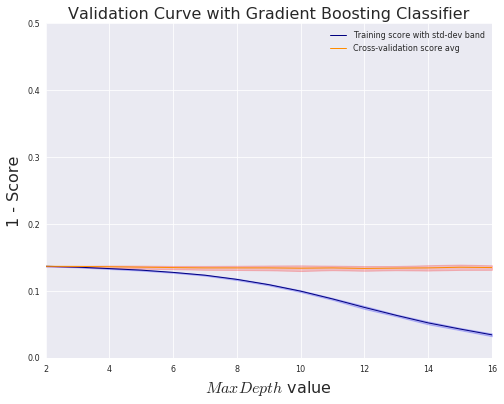
\includegraphics[width=1\linewidth]{figures/gradient-boosting/validation_curve_boosting_depth_series_f1}
        \caption{ Validation curve for the tree-depth hyperparameter of the Gradient Boosting Tree learner.
        The mean CV scores for the $1 - Accuracy$ score is shown for a CV run experiment on \cref{target2}}
        \label{fig:boosting_validation_curves_depth_trees}

    \end{center}
\end{figure}

\begin{figure}[h!]
    \begin{center}
        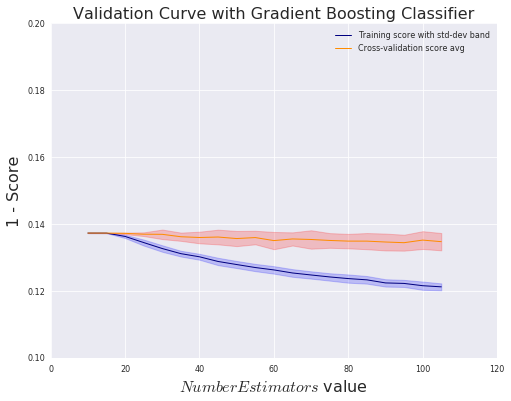
\includegraphics[width=1\linewidth]{figures/gradient-boosting/validation_curve_boosting_num_trees_series_f1}
            \caption{ Validation curve for the number of trees hyperparameter of the Gradient Boosting Tree learner. The mean CV scores for the $1 - Accuracy$ score is shown for a CV run experiment on \cref{target2}}
            \label{fig:boosting_validation_curves_num_trees}
    \end{center}
\end{figure}


Recall how these outcomes compare to \cref{figure:dtree_overfit_problem_2} and \cref{fig:random_forest_validation_curves_num_trees},
in which a tree's training error always improves as a result of an increase in the tree's depth.

Here, we see that the estimator is prone to overfitting when using a high $max depth$ value because the training deviates faster from the CV error when the depth is higher.
This acceleration is clear from the figure when we see that the CV score is invariant while the training error decreases.
At the same time the model differs to the Random Forest classifier in that the trees are not uncorrelated, because the $t$-th tree improves on the error of the model at $t$.
This is an effective difference in the models.

For the second experiment, the overfit is smaller, given that the relative difference in the CV score and the train score is smaller.

It is interesting to note that, for both cases, there is a very small gain in the CV error when varying the hyperparameters, as evidenced by the range of the scores.
Yet the decrease in CV score is slightly better for the second experiment and this situation is different to the case of the Random Forest learner, where the scores had a stronger improvement in the cross validated score.
The model seems to better fit the data compared to the Random Forest, since lower error rates are achieved, and it converges faster to a stable CV error where adding more trees or depth doesn't improve on the score.

At their optimal configuration, both setups reached CV score averages of at least $86.5\%$, with a maximum of $86.9\%$ for the learner with trees of 12 levels.
However, the optimal number of estimators for the CV and training sets were different, where 105 was the best configuration for the training score and 95 was the best average for the CV set.
Wit this, the relative difference in these best scores was of $1.5\%$.
It is not surprising that the relative difference of the best CV and training scores, for the maximum tree depth experiment was much higher with $11.5\%$, given this hyperparameter's influence to the model's complexity.

The outcomes here expose the drawbacks of this model which is more prone to overfitting and takes longer to fit when compared to the Random Forest algorithm.
Yet it gives better overall performance on the CV error, when the model is correctly calibrated.



%\subsection{Gradient Tree Boosting}
%
%%\todo{Move to appendix all necessary parts.}
%
%As explained before, the boosting methods build an ensemble model learned from other \textit{weaker} learners where decision trees are the most commonly used base models.
%
%This is the same for \textit{gradient tree boosting}, which is a small variant of the model in which
%
%This type of boosting algorithm was first introduced by Friedman, J., and the full details of the work can be found in Full details of this model can be found in \citep{friedman-gradientBoosting2001}.
%
%Using the same formulation as before, let $Tr$ be a set of tree models and $K$ the number of trees in $Tr$, then trees will be the parameters for this model and at step $m$ the output will be
%
%\begin{equation}
%\hat{y}^{(m)}= \sum_t^m \gamma_t h_t(x) , \ h_t \in Tr \ \forall t \in {0,\ldots,K}
%\end{equation}
%
%where $\gamma_t$ indexes the weight for each tree $h_t$.
%
%At each step, a new base learner is added to the model through $\gamma_{m+1}$ and $h_{m+1}(\cdot)$:
%
%\begin{equation}
%\hat{y}^{(m+1)} =  \hat{y}^{(m)} + \gamma_{m+1} h_{m+1}(x)
%\end{equation}
%
%in such a way that the loss function previously is minimized by the next best base learner:
%
%\begin{equation}\label{eq:boosting_iterative_minimization}
%h_{m+1}(\cdot) = \underset{h_{m+1},\gamma_{m+1}}{\mathrm{argmin}}  \sum_{i=1}^{n} L ( y_i, \hat{y_i}^{(m)} - \gamma_{m+1} h_{m+1}(x_i) )
%\end{equation}
%
%
%If we treat the tree's weight $\gamma$ as part of the weak learners hyper parameters, we can absorb that parameter and note each weak learner as
%
%$$\theta^{m+1}_{q(x)} \forall m in \{1,2,\ldots,K \}$$.
%
%This notation follows the one used in $\cref{section:decision_trees}$
%
%where we represent a generic tree in the form of
%
%\begin{equation}
%\theta_{q(x)} = \sum_{j=1}^J \theta_j I(x \in R_j)
%\end{equation}
%
%
%%Therefore the model results in,
%%
%%\begin{equation}
%%y = \sum_k f_t(x) , \ f_t \in Tr \ \forall t \in {0,\ldots,K}
%%\end{equation}
%
%
%with $\theta_j \in \mathbb{R} \ \forall j = 1,\ldots,J$ and $ \cup_{j=1}^J R_j$ a feature space partition.
%
%The function
%\begin{equation}
%q : X \mapsto \{1,\ldots,J\}
%\end{equation}
%
%denotes the mapping from samples to regions in the partition.
%
%In summary, this notation sets
%$${\{\theta_j, R_j\}}_{j=1}^J$$
%as the weak model's parameters and $J$ as a hyper-parameter.
%We know that finding the best partition of feature space is a non-trivial optimization problem since finding subset partitions satisfying a global condition is combinatorially hard.
%
%For the full model, the objective function would account for the relationships among the trees and we would have that
%
%\begin{equation}\label{eq:boosting-objfunction}
%Obj(\Theta) = \sum_i^n l(y_i,\hat{y}_i) + \sum_t^K R(\theta^m_{q(x)})
%\end{equation}
%%\footnote{In the formula \cref{eq:boosting-objfunction} }
%
%At the outer level view of the model,$\Theta$ is a parameter encoding all of the base trees' model information.
%For each base tree $\theta^m$ is the parameter associated to it and $R{\cdot}$ is a regulating function on the trees' complexity.
%
%This means that
%
%$$\Theta = \bigcup_{m \in {0,\ldots,K}} \theta^m \cup \theta_0$$
%
%The parameter $\Theta$ is not associated to any tree but reserved to characterize the whole ensemble.
%

%If an optimization routine were to collectively fit all the parameters in $\Theta$ to learn this model, we would have a very computational complex model.
%In practice this would result in an prohibitive cost.
%Instead, we rely on optimization heuristics which rely on first and second order approximations of the loss function at step $m$ to build on the next tree $m+1$.
%Smooth loss functions are then fundamental for this procedure to work such as in the Adaboost formulation.
%The \textit{boosting} optimization heuristic is explained in detail in \cref{appx:sec:boosting_optimization_heuristic}.
%
%
%As a concluding remark on boosting algorithms, there are two additional heuristics used to improve their generalization performance.
%The arguments in favor of these methods are rather experimental and not much theoretical, although their benefits are intuitive.
%The authors in~\citep{hastie-elemstatslearn} and~\citep{bishop-patternecognition} mention them because of their overall contribution to the generalization error.
%
%The first idea to reduce the overall variance of the algorithm is to subsample the data.
%This means that at each iteration, only a bootstrapped sample of the dataset will be selected to build the new weak learner.
%Samples from $\mathcal{T}$ which are not part of the bootstrapped sample are ignored when optimizing for the new learner at \cref{eq:boosting_iterative_minimization}.
%
%The motivation behind this is the same that as in Random Forest, where reducing the overall of available data to fit the new weak learner will most likely reduce the variance of the method.
%In practice, the rate of sampling will be supervised by a tuning parameter in the model.
%
%The other heuristic, which was found to be more experimentally important by~\citep{hastie-elemstatslearn}, is to successively apply a \textit{shrinkage} factor $v \in (0,1)$ to the new model.
%At step $m$, instead of letting the overall model be
%
%\begin{equation}
%\hat{y_i}^{(m)} = \hat{y_i}^{(m-1)} + \theta_m h_m(x_i)
%\end{equation}
%
% we multiply the shrinkage factor $v$ to the new learners before adding them to the overall model.
%
%In the literature this shrinkage factor is also called the \textit{learning rate} of the algorithm.
%Note that $v$ is reducing the movement of the algorithm in the direction of optimization provided by $\theta_t$ and $h_t$.
%In practice, this results in longer iterations needed to reach the algorithm's \textit{best} prediction rate.
%However, when this factor is combined with sub sampling, experiments have shown improvements in the overall generalization accuracy.


\subsection{Experiments}\label{subsection:boosting_experiments}


In this subsection, we explore on the task described in \cref{target4}, using Gradient Boosting classifiers and we compare the outcomes with the results outlined in \cref{subsection:random_forests_experiments}.
We set two experiments similar to the ones before, where we run two procedures: one with all available features and another without the top target-correlated ones.
In this setup though, we had a minor difference where, as before, it was characterized by the attributes used by our training dataset.

For the third experiment, we trained \textbf{only} with the best features extracted from the Random Forest's second experiment.
These were selected from the best-fit learner used from that case.

With this third variant, we expected to see how good of a performance can the gradient boosting classifier achieve, using only the top 30 features, as selected by best-fit random forest learner for the previous experiments.
% Even though
Doing this has a hypothetical trade-off between accuracy and procedure run-time, where we can gain speed in our fitting process by compromising some of the predictive power of the algorithm.

Once again, here we performed a cross validation procedure over the available hyperparameters of this classifier.
For the most part, these hyperparameters are the same as for the Random Forests learner.
Still, this model has some additional ones, which we outline in \cref{list:boosting_grid_search_params}.
For our CV procedure, we will be searching the best learner over a grid combination of all parameters.

\begin{itemize}

  \item The gradient descent's defined step size  --- [$step\_size$]
  % \item The number of rounds without loss function improvement required to early stop the fit  --- [early\_stopping]
  \item Minimum threshold for the sum of samples' Hessians at a given node.
  If a node's sum is smaller than this threshold then the fitting will stop  --- [$min\_leaf\_weight$]
\label{list:boosting_grid_search_params}
\end{itemize}


Using the same setup as before, we recorded the outcome of the three experiments' cross validation procedures.
The results were tabulated in terms of different metrics' scores, runtime, best resulting hyperparameters values and the top ten best features as selected by the best models.

A summary of the metrics and best hyperparameter values is given in \cref{tab:boosting_big_experiment_results}.

\begin{table}[!htb]
\caption{Table of best results comparing three 10-fold full grid cross validation procedures with a Gradient Boosting Classifier for \cref{target4}.  All relevant scores, best hyperparameter values and run-time are shown for both experiments.}
\label{tab:boosting_big_experiment_results}
\centering
\begin{tabular*}{0.9\textwidth}{@{\extracolsep{\fill} }  l l l l l }
%{|p{2cm}|p{2cm}|p{1.5cm}|p{1cm}|p{1.5cm}}
\toprule
Result & Experiment 1 & Experiment 2 & Experiment 3 \\
\midrule
Running time (s)      & 2993  & 1972   &  204   \\
CV $F1$ score         & 0.314 & 0.319  & 0.354  \\
CV $Accuracy$ score   & 0.889 & 0.843  & 0.8327 \\
CV $Precision$ score  & 0.209 & 0.217  & 0.249  \\
CV $Recall$ score     & 0.629 & 0.601  & 0.607  \\
CV $ROC AUC$ score    & 0.884 & 0.880  & 0.831  \\
CV $Logloss$ score    & 0.524 & 0.337  & 0.399  \\
$balanced$            & False & False  & False  \\
% early\_stopping  & 5 &  5 & 5 \\
$max\_depth$          & 15    & 15     & 12 \\
$num\_trees$          & 250   & 300    & 120 \\
$min\_leaf\_weight$   & 2     & 5      & 10 \\
$min\_loss$           & 10    & 1      & 0.01 \\
$step\_size$          & 0.01  & 0.1    & 1 \\
$max\_features$ (\%)  & 80    & 75     & 10 \\
\bottomrule
\end{tabular*}
\end{table}

The first notable fact from the results is how fast the last experiment is, compared to the first two.
Training the model was much faster, with almost 3 minutes to complete the full procedure whilst the others had at minimum 20 minutes to do so.
We see that the information from the top 30 features of the RF models was efficiently used in this boosting experiment and that this feature reduction considerably sped up the learner's runtime.
This improvement should not be surprising then, as we have limited the amount of available features to use, thus decreasing the necessary computer resources to compute the fit.
% However, this conclusion might seem

The second interesting fact from the outcome is that the model seems to be more overfit, when compared to Random Forest experiments.
This is specially significant in the first two, where very complex models were chosen from the procedure, with a depth of 15 levels and at least 250 trees for both.
However, this is not the last model's case though, where a more simple model resulted with a depth of only two levels and 120 trees grown.

The same applies for the $max\_features$ and $min\_leaf\_weight$ hyperparameters, for which lower complexity values resulted form the last CV procedure.
There is difficulty though in establishing which of them had the most weight in an underweight model.

When analyzing the $F1$ score of the experiments, we find ourselves with a scenario which is not that different.
We see that the last procedure improved on the first two experiments in more than $10\%$, using this score and in an almost $20\%$ increase in the precision score.
This suggests that the first two models were overfitting the training set and by using the top random forest features, we strongly improved on the $F1$ performance.
Finally, when compared to the Random Forest's experiments, we see that the boosting models performed near to the top $F1$ value of $37\%$ achieved in the Random Forest experiments.
The worst relative difference for all models, to this value, was of $17\%$ at most and $4.5\%$ at least.

Still, for that case, the top Random Forest's $F1$ score was attained in the first experiment, where we made use of the highly target-correlated features.
This is then a remarkable performance for boosting learners which were not trained on this attributes and still achieved similar or higher scores.

We also notice that the third model lacked the same strength for the $ROC AUC$ score.
Here, the first model reached a score of almost $90\%$, whereas the third model had a poorer performance of $83\%$.
Still, the lowest value for all experiments is more than satisfactory for the prediction task.

With these results, and due to the difference in $ROC AUC$ vs. $F1$ scores, there is no clear indication as to which configuration is better across all experiments.

Below we introduce the learner's selection of best features for each experiment.
Note that the last selection will have a very similar configuration to the top Random Forest features, since it selects 10 features of the available 30 used to train the model.
This outcome is presented in \cref{tab:boosting_big_experiment_best_features}, where the top 10 features for each experiment are shown.


\begin{table}[ht]
    \centering
    \caption{A representation of the top features that resulted from the Gradient Boosting procedure on two experiments of  \cref{target4}. }
    \label{tab:boosting_big_experiment_best_features}
    \resizebox{\textwidth}{!}{%
        \begin{tabular}{@{}llll@{}}
            \toprule
            & \multicolumn{3}{l}{Top Features}                                                                   \\ \midrule
            \multicolumn{1}{l|}{\multirow{4}{*}{First Experiment}}  & Call Count Antenna\_0 & Mobility Diameter  & Mobility Diameter Weeknight  \\
            \multicolumn{1}{l|}{}                                   &  Call Count Weeknight Antenna\_0 &  Call Count Antenna\_1  & Call Count Antenna\_2  \\
            \multicolumn{1}{l|}{}                                   &   TimeWeekDay In Month\_08  & Call Count Weeknight Antenna\_2 &  TimeWeekDay Out Month\_09  \\
            \multicolumn{1}{l|}{}                                   &  & TimeWeekDay Out Month\_12  &       \\ \midrule
            \multicolumn{1}{l|}{\multirow{4}{*}{Second Experiment}} & Mobility Diameter  & Mobility Diameter Weeknight   &  Call Count Antenna\_0   \\
            \multicolumn{1}{l|}{}                                   &  Call Count Weeknight Antenna\_0 & Call Count Antenna\_0   & TimeWeekDay In Month\_09   \\
            \multicolumn{1}{l|}{}                                   &  TimeWeekDay Out Month\_09  & TimeWeekDay Out Month\_12   &  TimeWeekDay Out Vul Month\_08 \\
            \multicolumn{1}{l|}{}                                   &   &  TimeWeekDay In Month\_10  &              \\ \midrule
           \multicolumn{1}{l|}{\multirow{4}{*}{Third Experiment}} &  TimeWeekDay In Vul Month\_09 & CallsWeekDay In  Month\_09   &  TimeWeekDay Out Vul Month\_12   \\
            \multicolumn{1}{l|}{}                                   &  Mobility Diameter Weeknight  & Call Count Weeknight Antenna\_0   & CallsWeekDay Out  Month\_09    \\
            \multicolumn{1}{l|}{}                                   &  CallsWeekDay In Vul  Month\_08 &  TimeWeekDay In Vul  Month\_08  &  TimeWeekDay Out  Month\_08  \\
            \multicolumn{1}{l|}{}                                   &   & TimeWeekDay In  Month\_12 &   \\
            \midrule
            \end{tabular}%
    }
\end{table}


The top features list shows us the importance of mobility diameter in both cases.
We see that both weeknight and all-week user's mobility, are deemed relevant to detect their past endemic condition.
This outcome confirms what was seen in \cref{tab:random_forest_big_experiment_best_features} where these attributes were, in general, performing.

As expected, in all cases we see that there are a number of features logging vulnerable interactions of users living in non-endemic regions.
The same can be said about the call volume features, which are selected as important, both in the number and times of calls.
Unluckily, we can't determine its relationship to the target variable in the sense that it might equally affect in both a positive and negative way.
% Phone behavior might differ along
% Where user phone behavior

These results are in line with the assumptions we made when we constructed the risk maps in \cref{section:riskmaps}.
The direction and duration of calls, and the number of occurrences of these are all relevant predictors in the problem of tagging users that moved out of the endemic region.

Once again, we see there are more features of earlier month interactions, such as August and September.
At the same time, the only other month appearing is December.
This could be indicative of familiar relations as it is a month which coincides with festivities and family reunions.

However, we understand that this best-features methodology is constructed over a heuristic, so there doesn't seem to be any clear indication over which type of CDR interaction has better predictive power.

The analysis here confirms the relevance of CDR information in tagging long-term migrations.
Experimental results show satisfactory scores across different metrics and for a highly imbalanced class.
Also, top features are in line with the assumptions on which the risk maps were constructed.
%Top features are related to the vulnerability and to the users mobility


\section{Benchmark Classifier: Naive Bayes}\label{section:naive_bayes}

The Naive Bayes model encompasses a group of simple and computationally efficient algorithms which are built with a strong statistical assumption of independence among the features.
Even though this belief is in practice wrong, the model still achieves acceptable classification rates for some problems.
In addition, it does not suffer in problems of high-dimensionality, where $p >> n$ i.e.\ there are more attributes than samples in the data.

It is presented in this work for the purpose of providing a benchmark algorithm.
In practice it is expected that the classification rate achieved by this model serves as a baseline for other, more complex, learners.

The benefits of the algorithm include having linear complexity in the number of features and samples $O(d+n)$, so it can be easily extended to \textit{large} problem implementations.
Furthermore, its maximum-likelihood estimation of the parameters has a closed form solution which is faster to compute over other iterative methods such as techniques using gradient descent or other similar iterative optimization routines.

Let $x = (x_1,\ldots,x_p)$ be any given data sample and $C_k$ be one of $K$ possible output classes of a classification problem.
We take $p(C_k \mid x)$ to be the class posterior probability of this class given the sample.

In \cref{ch:machineLearning}
we have used
\begin{equation}
\label{eq:posteriorProbabilties}
p(C_k| x) = \frac{P(x|C_k)P(C_k)}{P(x)}
\end{equation}


and argued that if our data is given, then our model can only improve the posterior probability by optimizing $P(x|C_k)P(C_k)$ which is just the joint probability of the sample and the class.

Here we can approximate the posterior as

\begin{equation}
\label{eq:posteriorProbabilityDecomposition1}
P(C_k \mid x) \approx p(C_k) * \prod_{j=1}^{p}  P(x_j \mid \bigcap_{k=j+1}^{p} x_k \cap C_k)
\end{equation}


We now impose a strong independence assumption among features, given the target class, to let the conditional probability factors become the probability of each feature. %This assumption is what gives the model its

This yields a posterior probability which depends only on the prior probability and on the individual likelihood of each feature.

\begin{equation}\label{eq:posteriorProbabilityDecomposition2}
P(C_k \mid x) \approx p(C_k) * \prod_{j=1}^{p}  P(x_j | C_k)
\end{equation}
As we have said before, the parameters of the model can only reweigh the likelihood factors, so if we look to maximize the posterior probability, our final estimate of the posterior will take the following form.

\begin{equation}\label{eq:posteriorProbabilityDecomposition3}
P(C_k \mid x) = \frac{1}{Z} p(C_k) * \prod_{j=1}^{p}  P(x_j | C_k)
\end{equation}

where in the equation $Z = p(x)$ is a scaling factor and is fixed to the dataset.

In practice, the model will stem into different algorithms where each variant will have a different probabilistic assumption on the likelihoods $p(x_j \mid C_k)$ of the model and on the priors $p(C_k)$.
It is common to choose among these by  using non-parametric density estimations from the training data or by setting parametric assumptions on the data distribution, such as being distributed from an exponential distribution family such as a Gaussian, Bernoulli or Multinomial distribution.

Different choices will certainly lead to different cross validation scores among problems.
Altogether, these choices can be treated as part our model's hyperparameters and the best one can be selected with our CV procedure.
%Indeed,

Finally, the output class for a given sample will be given by taking the class $k'$ which maximizes the probability $P(C_k' \mid x)$.

\subsection{Experiments}\label{subsection:naive_bayes_experiments}

Here we present a very brief outline of this algorithm's performance on our general problem.
Without going in to depth on the specifics of the experiments, we ran the classifier in a cross validation procedure against all of the four tasks outlined in \cref{long_term}, and using the same $Accuracy$, $F1$ and $ROC AUC$ classifier scores as in other method's experiment runs.
We took advantage of this method's fast training runtime to rapidly evaluate all tasks on this algorithm.
% The speed small time needed to fit this classifier on a large dataset.
The results were composed into \cref{tab:naive_bays_experiment_results} and are shown to highlight two aspects of the method: its lower performance when compared to other previous methods, and the algorithm's fast run-time.


\begin{table}[!htb]
\caption{Table comparing cross validated results
of best fit learners, comparing all 8-fold cross validation procedures on a Naive Bayes classifier. Here a Multinomial prior distribution was used and the relevant classification scores are shown}
\label{tab:naive_bays_experiment_results}
\centering
\begin{tabular*}{0.9\textwidth}{@{\extracolsep{\fill} }  l l l l l }
%{|p{2cm}|p{2cm}|p{1.5cm}|p{1cm}|p{1.5cm}}
\toprule
Measure & Problem 1 & Problem 2 & Problem 3 & Problem 4  \\
\midrule
Running time (s)        & 125    &  121   &  105     &  85     \\
CV $Accuracy$ score     & 0.842  & 0.649  &  0.658   &  0.852   \\
CV $F1$ score           & 0.753  & 0.313  &  0.457   &  0.626   \\
CV $ROC AUC$ score      & 0.827  & 0.617  &  0.635   &  0.768   \\

\bottomrule
\end{tabular*}
\end{table}
